\documentclass[11pt]{article}
\usepackage{amsmath, amscd, amssymb, amsthm}
% \usepackage{diagrams}
\usepackage{color}
\usepackage{graphicx, psfrag, tikz}
\usepackage[all]{xy}
\usepackage[margin=1.1in]{geometry}

\usepackage{enumitem,kantlipsum}
\usetikzlibrary{arrows.meta}
\usetikzlibrary{calc,patterns,angles,quotes}
%\renewcommand{\baselinestretch}{1.17}
\usepackage{chemformula}

\newtheorem{theorem}{Theorem}[section]
\newtheorem{lemma}[theorem]{Lemma} 
\newtheorem{proposition}[theorem]{Proposition}
\newtheorem{corollary}[theorem]{Corollary}
\theoremstyle{definition} 
\newtheorem{definition}[theorem]{Definition}
\newtheorem{conjecture}[theorem]{Conjecture}
\newtheorem{remark}[theorem]{Remark}
\newtheorem{example}[theorem]{Example}

\begin{document}
\begin{center}
\textbf{Math 309 Homework 3}\\
(6 problems)
\end{center}
\vspace{0.15in}


\begin{enumerate}[leftmargin=*]

\item For simplicity, in this problem you can assume $x(t)$ is a scalar valued function, i.e. not vector valued, (though everything here works in exactly the same way even if $x(t)$ is a vector valued function).

\begin{itemize}
\item [(a)] Show that if $x^{(1)}(t)$ and $x^{(2)}(t)$ are solutions to a homogeneous linear first order equation, i.e. an equation of the form $x'=p(t)x$, then $x(t)=c_1x^{(1)}(t)+c_2x^{(2)}(t)$ is also a solution to $x'=p(t)x$.\\

\item [(b)] Now suppose $x^{(1)}(t)$ and $x^{(2)}(t)$ are nonzero solutions to the following homogeneous, but nonlinear, first order equation,
\[
x' = x^2.
\] 
Show that $x=x^{(1)}(t)+x^{(2)}(t)$ is not a solution to the above equation $x'=x^2$.\\

\item [(c)] Now suppose $x^{(1)}(t)$ and $x^{(2)}(t)$ are solutions to the following linear, but nonhomogeneous, first order equation,
\[
x'=x+2.
\]
Show that $x=x^{(1)}(t)+x^{(2)}(t)$ is not a solution to the above equation $x'=x+2$.  This $x$ is actually a solution to a different equation, and what is that equation?  \\
\end{itemize}

 \item  (Continuation of HW2 \#3) In HW2, \#3, we solved the below system of equations,
\[
\begin{array}{lll}
x_1' & = & x_1-2x_2  \\
x_2' & = & 3x_1-4x_2
\end{array},
\]
by writing this system as a single 2nd order equation and solving that 2nd order equation first. 

\begin{itemize}
\item [(a)] Now forget about writing the system as a 2nd order equation.   Just find the general solution to the above first order system $x'=Ax$ directly by finding the eigenvalues and eigenvectors fo the coefficient matrix $A$.

 \item [(b)]  Describe the behaviors of the solution as $t\to \infty$ and as $t\to - \infty$, (i.e. are solutions $x(t)$ going to $0$ or $\infty$?)
 
\item [(c)] Draw a few trajectories of solutions in the $x_1$-$x_2$ plane.  Draw the trajectories parallel to the eigenvectors and also include a couple of trajectories that are not parallel to the the eigenvectors.  Indicate the direction of flow by drawing an arrow on each trajectory.\\
\end{itemize}



\item (Continuation of HW3 \#2) 
\begin{itemize} 
\item [(a)] Find the solution to the above system of equations given the following initial condition
\[
x(0)=\left[
\begin{array}{c}
-1 \\
-2
\end{array}
\right]
\]
\item [(b)] Plot the point $x(0)$ on the $x_1$-$x_2$ plane.
\item [(c)] Draw the trajectory of the solution to part (a) on the $x_1$-$x_2$ plane for $t\in [0,\infty)$.  Indicate the direction of flow. 
\item [(d)] Plot the point $x(1)$ on your drawing in part (c).  \\
\end{itemize}

\item (Rolling down a potential hill, a continuation of HW2 \#6)
In HW2, \#6b, we wrote down the following system describing the motion of the particle
\[
\left[\begin{array}{l} x'\\ p' \end{array}\right]=A  \left[\begin{array}{l} x\\ p\end{array}\right],\quad \text{ where } A= \left[\begin{array}{cc} 0& 1/m  \\ 2/5 & 0 \end{array}\right].\]

\begin{itemize}
\item[(a)] Find the general solution, $\left[\begin{array}{l} x(t) \\ p(t) \end{array}\right]$, to this system by finding the eigenvalues and eigenvectors of $A$.  (The answer you get in the end should be the same as that in HW2 \#6a.) \\

\item[(b)] Suppose $x(0)=0$ and $p(0)=0$.  Find the solution $\left[\begin{array}{l} x(t) \\ p(t) \end{array}\right]$ subject to this initial condition.\\

\item[(c)] Again $x(0)=0$ and $p(0)=m$ (i.e. initial velocity points to the right).  Find the solution $\left[\begin{array}{l} x(t) \\ p(t) \end{array}\right]$ subject to this initial condition.  

\item [(d)] What is the behavior of the solution in part (c) as $t\to \infty$?   (That is, are solutions  going to $0$ or $\infty$?)

\item [(e)] Let $m=1$.  Draw the trajectory of solution in part (c) for  for $t\in [0, \infty)$ in the $x$-$p$ plane and remember to indicate the direction of flow.  \\
\end{itemize}

\item (Pendulum, a continuation of HW1 \#8) In HW1 \#8, we discussed  that the equation of motion for a frictionless pendulum of bob mass $m$ and rod length $L$ is 
\[ 
\theta''(t) =-\frac{g}{L}\sin \theta.
\]
This is a nonlinear equation, and we linearized it in HW1 by considering very small $\theta\approx 0$, in which case $\sin\theta\approx \theta$.  

Now let's linearize it near a different point by considering $\theta \approx \pi$, so the bob of the pendulum is near the very top as pictured below.  In this case, by considering a Taylor expansion of $\sin \theta$ around $\pi$, we get that $\sin \theta\approx -(\theta-\pi)$.  Then we get that for $\theta\approx \pi$, we can approximate the above nonlinear equation by the following linearized equation
\[
\theta''(t)=\frac{g}{L} (\theta-\pi).
\]
Now let $\tilde \theta=\theta-\pi$, so when $\theta=\pi$,  we have $\tilde \theta=0$.  Then the above equation becomes 
\[
\tilde \theta'' =\frac{g}{L}\tilde \theta.
\]

For the rest of this problem, we only consider this very last linearized equation in $\tilde \theta$.

\begin{center}
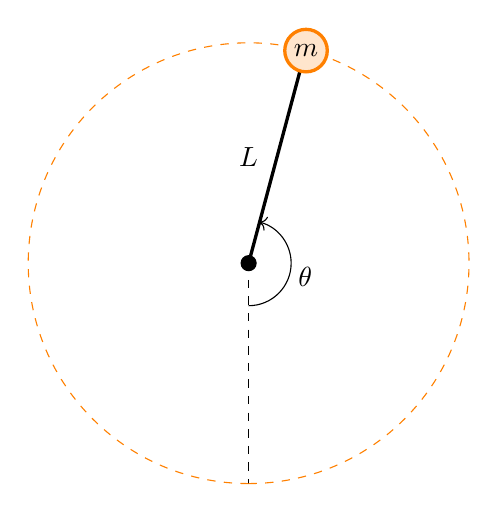
\begin{tikzpicture}[scale=0.9]

\draw[black,fill=black] (0,0) circle (0.7ex);
\draw [dashed] (0,0) -- (0, -3.11);
  \draw[dashed, orange] (0, -3.11) arc (-90: 74: 3.11);
      \draw[dashed, orange] (0, -3.11) arc (-90: -284: 3.11);

 \draw[very thick] (0,0)--(0.73, 2.73);
 \draw[orange, very thick,fill=orange!20] (0.81, 3) circle (0.3cm);
 
 \draw [->](0,-0.6) arc (-90:75:0.6);
 \node at (0.8, -0.2) {$\theta$};
  \node at (0, 1.5) {$L$};
  \node at (0.81, 3) {$m$};

          
\end{tikzpicture}
\end{center}

\begin{itemize}
\item [(a)] Denote by  $\omega(t)=\frac{d\theta(t)}{dt}$.  Write the above linearized equation in $\tilde \theta$ as a system of first order equations
\[
\left[\begin{array}{l} \tilde \theta'\\ \omega' \end{array}\right]=A  \left[\begin{array}{l} \tilde \theta\\ \omega \end{array}\right].
\]

\item[(b)] Find the general solution to the system in part (a) by finding the eigenvalues and eigenvectors of $A$.

\item[(c)] Now set $\frac{g}{L}=1$.   Draw a few trajectories of solutions in the $\tilde \theta$-$\omega$ plane.  Draw the trajectories parallel to the eigenvectors and also include a couple of trajectories that are not parallel to the the eigenvectors.  Indicate the direction of flow by drawing an arrow on each trajectory.

\item[(d)] Again keep $\frac{g}{L}=1$.  Draw the trajectory determined by the initial condition $\tilde \theta(0)=0$ and $\omega(0)=1$ for $t\in [0,\infty)$ in the $\tilde \theta$-$\omega$ plane.  Then on the same plane, also draw the trajectory determined by the initial condition $\tilde \theta(0)=0.3$ and $\omega(0)=0$ for $t\in [0,\infty)$  
\end{itemize}

\item Consider the following system 
\[
x'=\left[
\begin{array}{cc}
2 & -1\\
3 & -2
\end{array}\right]x.
\]
\begin{itemize}
\item [(a)] Find the general solution by finding the eigenvalues and eigenvectors of the coefficient matrix.
\item [(b)] Draw a few trajectories of solutions in the $x_1$-$x_2$ plane.  Draw the trajectories parallel to the eigenvectors and also include a couple of trajectories that are not parallel to the the eigenvectors.    Indicate the direction of flow by drawing an arrow on each trajectory.
\item [(c)] Draw the trajectory determined by the initial condition $x_1(0)=2$ and $x_2(0)=1$ for $t\in [0,\infty)$ in the $x_1$-$x_2$ plane.
\end{itemize}


\end{enumerate}





\end{document}
